\documentclass{report}
\usepackage{lmodern}
\usepackage{amssymb,amsmath}
\usepackage{dsfont}
\usepackage{graphicx}
\usepackage{ifxetex,ifluatex}
\usepackage{bm}
\usepackage{fixltx2e} % provides \textsubscript
\ifnum 0\ifxetex 1\fi\ifluatex 1\fi=0 % if pdftex
  \usepackage[T1]{fontenc}
  \usepackage[utf8]{inputenc}
\else % if luatex or xelatex
  \ifxetex
    \usepackage{mathspec}
  \else
    \usepackage{fontspec}
  \fi
  \defaultfontfeatures{Ligatures=TeX,Scale=MatchLowercase}
\fi
% use upquote if available, for straight quotes in verbatim environments
\IfFileExists{upquote.sty}{\usepackage{upquote}}{}
% use microtype if available
\IfFileExists{microtype.sty}{%
\usepackage[]{microtype}
\UseMicrotypeSet[protrusion]{basicmath} % disable protrusion for tt fonts
}{}
\PassOptionsToPackage{hyphens}{url} % url is loaded by hyperref
\usepackage[unicode=true]{hyperref}
\hypersetup{
            pdfborder={0 0 0},
            breaklinks=true}
\urlstyle{same}  % don't use monospace font for urls
\IfFileExists{parskip.sty}{%
\usepackage{parskip}
}{% else
\setlength{\parindent}{0pt}
\setlength{\parskip}{6pt plus 2pt minus 1pt}
}
\setlength{\emergencystretch}{3em}  % prevent overfull lines
\providecommand{\tightlist}{%
  \setlength{\itemsep}{0pt}\setlength{\parskip}{0pt}}
\setcounter{secnumdepth}{0}
% Redefines (sub)paragraphs to behave more like sections
\ifx\paragraph\undefined\else
\let\oldparagraph\paragraph
\renewcommand{\paragraph}[1]{\oldparagraph{#1}\mbox{}}
\fi
\ifx\subparagraph\undefined\else
\let\oldsubparagraph\subparagraph
\renewcommand{\subparagraph}[1]{\oldsubparagraph{#1}\mbox{}}
\fi

% set default figure placement to htbp
\makeatletter
\def\fps@figure{htbp}
\makeatother


\def\doubleunderline#1{\underline{\underline{#1}}}

\date{}

\usepackage{tcolorbox}
\usepackage{capt-of}
\usepackage{float}

\begin{document}


\chapter{Introduzione}
Quali sono gli indici che mi dicono se ho sviluppato un buon modello? +
adattamento dei dati (fit dei dati) + semplicità del modello (numero dei
parametri). Un modello serve per capire di più riguardo ad un fenomeno e
non per complicarlo (parsimonia).

Qual è la differenza tra modello matematico e statistico?
\(\rightarrow\) Incertezza. Il modello statistico è caratterizzato
dall'errore. L'errore considera la variazione individuale.
\(\rightarrow\) Variabili esplicative che possono essere considerate per
migliorare il modello (quindi diminuire l'errore). \(\rightarrow\) Nel
caso stocastico errori nel rapporto campione-popolazione.

Il lavoro nel costruire un modello statistico sta sia nel diminuire
l'errore ma anche nel capire da dove nasce. 

Come nasce l'elaborazione di un modello statistico?

\begin{itemize}
	\tightlist
	\item
	Teoria, Ovvero formulazione di ipotesi, scoperta di relazion empiriche
	o rapporti di causa effetto tra variabili. Individuazione delle
	variabili esplicative.
	\item
	Dati. Capire quale metodo di raccolta utilizzare in base anche alla
	disponibilità economica che si ha per sviluppare il modello.
	Trattamenti preliminari (pulizia ecc.) e poi tornare al modello.
	Tenere conto dell'eterogeneità dei dati (es. considerando per esempio
	il livello di pericolosità delle acque di un lago, se valutiamo tutte
	le particelle nella loro totalità potremmo non concludere che le acque
	sono pericolose, questo potrebbe infatti risultare valido nella sua
	totalità ma magari identifichiamo delle zone in cui avvengono più
	morti rispetto alla normalità. Questo perché ci potrebbero essere
	delle zone maggiormente inquinate che non emergono da un'analisi
	totale delle acque. Quindi considerare anche campionamenti di questo
	tipo , utilizzare tutti i dati potrebbe non dirci nulla). In questa
	fase rientra anche una prima analisi preliminare dei dati.
	\item
	Specificazione del modello (Probabilistico o descrittivo)
	\item
	Stima dei parametri e verifica dell'adattabilità ai dati
	\item
	Utilizzo
\end{itemize}

Ripetere più volte (se necessario).

\emph{Oss.} Oggi un problema nella costruzione di un modello è anche la
privacy. Ci sono modelli che potrebbero essere molto interessanti ma non
si possono elaborare per problemi di privacy. Quindi devo usare il
modello che ho per correggere i dati in questo senso (Teoria
\(\rightarrow\) Dati). Vale però anche il contrario, ovvero i Dati
aiutano nell costruzione di un modello
(\(\Rightarrow \text{Dati} \rightarrow \text{Teoria}\))

Il modello di base è il \emph{modello di regressione}. La regressione
può essere \emph{semplice}, \emph{multipla} o \emph{multivariata}.
\emph{Semplice}, se si ha una sola variabile dipendente ed una sola
variabile esplicativa. \emph{Multipla}, se si hanno più variabili
esplicative e una sola dipendente. \emph{Multivariata}, se si ha più di
una variabile esplicativa e più di una variabile dipendente.

\textbf{Stima}, ovvero trovare i parametri per il modello. Uno dei
metodi di stima è quello di \emph{regressione lineare}.

\textbf{Verifica} dei risultati sia in termini descrittivi (adattamento
ai dati), poi test statistici sulla significatività. Se la verifica non
conduce ad un rifiuto del modello stimato allora lo si utilizza
altrimenti si torna alla fase di specificazione. 


\chapter{Modello Lineare Classico} 
Il modo più generale per esprimere una legge di regressione lineare secondo il modello classico è:

\begin{equation}
\underline{Y} = \doubleunderline{X} \cdot \underline{b} + \underline{\varepsilon}
\end{equation}
con
\begin{equation}
\underline{Y} = 
\begin{pmatrix}
y_1 \\ 
. \\ 
. \\ 
. \\ 
y_n
\end{pmatrix}
\quad
\doubleunderline{X} = \begin{pmatrix}
x_{1,1} & x_{1,2} & \dots & x_{1,k} \\ 
x_{2,1} & \dots & \dots &  \\ 
\vdots &  & \ddots & \vdots \\ 
x_{n,1} & \dots &  & x_{n,k}
\end{pmatrix} 
\quad
\underline{b} = \begin{pmatrix}
b_0 \\ 
. \\ 
. \\ 
. \\ 
b_n
\end{pmatrix} 
\quad
\underline{\varepsilon} = \begin{pmatrix}
\varepsilon_0 \\ 
. \\ 
. \\ 
. \\ 
\varepsilon_n
\end{pmatrix} 
\end{equation}
dove $\underline{b}$ rappresenta il vettore dei regressori, mentre $\underline{\varepsilon}$ quello degli errori per ciascuna osservazione. Questo modello si basa su alcune ipotesi che analizziamo di seguito.

\subsection{Ipotesi di Linearità}
Secondo questa ipotesi, sia le variabili esplicative del modello (i valori della matrice $\doubleunderline{X}$) sia i parametri $\underline{b}$ sono lineari.

\subsection{Ipotesi di Non Sistematicità degli Errori}
Quest'ipotesi sostiene che la distribuzione di probabilità condizionata di ogni errore $\varepsilon_i$ dato il corrispondente vettore delle variabili esplicative $\underline{X}_i$ è centrata in zero, cioè:
\begin{equation}
E\left(\varepsilon_i|\underline{X}_i\right) = 0
\end{equation}
Di conseguenza la distribuzione della variabile dipendente è data da:
\begin{equation}
E\left(\underline{y}|\doubleunderline{X}\right) = \doubleunderline{X}\ \underline{b}
\end{equation}

\subsection{Ipotesi di Sfericità degli Errori}
Per quest'ipotesi valgono le seguenti:
\begin{enumerate}
	\item Ipotesi di \textbf{omoschedasticità}, ovvero la  variabilità  dell'effetto  di  tutti  i  fattori  non  rilevati  e/o  non  rilevabili  non  dipende  dai 
	valori dei regressori. Quindi:
	\begin{equation}
	V(e \vert x_1, \dots, x_n) = \sigma^2 \quad \Rightarrow V(Y \vert x_1, \dots, x_n) = \sigma^2
	\end{equation}
	\item Ipotesi di \textbf{incorrelazione}, ovvero gli  effetti su y dei  fattori  non  rilevati $\varepsilon$  per  l'osservazione i non  dipendono  da  quelli relativi all'osservazione j. Quindi:
	\begin{equation}
	Cov(\varepsilon_i, \varepsilon_j) = 0 \quad \forall i, j
	\end{equation}
	dove $\varepsilon_i$ e $\varepsilon_j$ sono appunto il valore delle variabili aleatorie per le osservazioni $i$ e $j$.
	\item Gli errori devono essere distribuiti in modo normale con media zero e varianza $\sigma^2$:
	\begin{equation}
	\varepsilon \sim N(0,\sigma^2)
	\end{equation}
\end{enumerate}

A questo punto se abbiamo tante osservazioni la situazione diventa la seguente:

Le condizioni ipotizzate prima sulle singole osservazioni del modello continuano a valere e possono essere riscritte in maniera più compatta come segue:
\begin{enumerate}
	\item E($\underline{\varepsilon}$) = 0
	\item V($\underline{\varepsilon}$) = E($\underline{\varepsilon}$, $\underline{\varepsilon'}$) = $\doubleunderline{\Sigma}$ = $\sigma^2 \mathds{1}_n$ 
\end{enumerate}


\subsection{Ipotesi di Non Stocasticità delle Variabili Esplicative}
Si suppone che i valori delle variabili esplicative $\underline{x}_j$ siano fissi e non soggetti a fluttuazioni stocastiche. Di conseguenza vale:
\begin{equation}
E(\doubleunderline{X}) = \doubleunderline{X}
\end{equation}
Ossia il valore di aspettazione della matrice delle covariate è la matrice stessa. Inoltre la correlazione tra questa e il vettore degli errori è nulla, cioè:
\begin{equation}
cov(\doubleunderline{X},\underline{\varepsilon}) = 0
\end{equation}

\subsection{Ipotesi di Non Collinearità delle Variabili Esplicative}
I vettori delle variabili esplicative contenuti nella matrice $\doubleunderline{X}$ sono linearmente indipendenti. La matrice $\doubleunderline{X}$ ha rango pieno, pari al numero delle covariate più uno dovuto al vettore costante, cioè:
\begin{equation}
Rank(\doubleunderline{X}) = p + 1
\end{equation}
Di conseguenza, la matrice ha determinante non nullo, è invertibile e il prodotto $\doubleunderline{X}\cdot\doubleunderline{X}^T$ è definito.

\subsection{Ipotesi sulla Numerosità della popolazione}
Si suppone che il numero di eventi nel campione sia maggiore della numero di covariate (più uno a causa del vettore costante):
\begin{equation}
n > p + 1
\end{equation}
Questo garantisce che la matrice $\doubleunderline{X} \cdot \doubleunderline{X}^T$ abbia un'unica inversa, dunque la soluzione al problema di regressione sia unica.


\section{Estimatori}

Un'estimatore è una funzione da applicare su un certo campione di dati preso in maniera casuale dalla popolazione. La stima è il valore numerico che l'estimatore assume quando viene calcolato sul set. Ogni estimatore può essere classificato sulla base di tre criteri.

\subsection{Correttezza (Unbiasedness)}
Lo stimatore può essere applicato su diversi campioni casuali. Perchè sia un buon estimatore, ci si aspetta che la distribuzione dei suoi valori sia centrata sulla stima esatta che avrebbe sulla popolazione, cioè:
\begin{equation}
E(\hat{\mu}_Y) = \mu_Y
\end{equation}

dove $Y$ è la popolazione considerata, $\hat{\mu}_Y$ è l'estimatore applicato su un campione e $\mu_Y$ è l'estimatore applicato alla popolazione. Se un'estimatore possiede questa proprietà è detto corretto o unbiased, altrimento è detto scorretto o biased.

\subsection{Consistenza (Consistency)}
Un' estimatore è detto consistente se all'aumentare della dimensione del campione su cui viene applicato, questo tende ad assumere il valore vero. Ciò si può scrivere come:
\begin{equation}
\hat{\mu}_Y \xrightarrow{p} \mu_Y
\end{equation}

\subsection{Efficienza (Efficiency)}
Siano $\tilde{\mu}_Y$ e $\hat{\mu}_Y$ due estimatori della stessa quantità $\mu_Y$, entrambi corretti. Il criterio dell'efficienza dice che per scegliere quale estimatore tra i due sia migliore, si guarda alla larghezza della loro distribuzione (cioè alla loro varianza): l'estimatore con varianza minore è quello più efficiente, cioè:
\begin{equation}
var(\hat{\mu}_Y) < var(\tilde{\mu}_Y)
\end{equation}
\section{Metodo dei Minimi Quadrati}


Come metodo di stima dei parametri $b$ si può utilizzare il \textit{metodo dei minimi quadrati}.

Nell'ipotesi di perfetta dipendenza lineare tra $Y$e gli $n$ regressori è possibile, facendo un campione di osservazioni, stimare i valori \underline{teorici} previsti per la variabile dipendente $y$ per tutte le unità del campione. Facendo la differenza tra questi valori teorici previsti e quelli empirici che risultano dall'osservazione si definiscono i residui come:
\begin{equation}
\underline{e} = \underline{y} - \underline{y'} = \underline{y} - \doubleunderline{X} \cdot \underline{b}
\label{eq: residui}
\end{equation}
dove con $\underline{y'}$ si è appunto indicato il vettore dei valori teorici previsti facendo una stima di $b$ sul campione.
\begin{equation}
y'_i = b_0 + b_1 x_{1i} + b_2 \dots + b_n x_{ni} \quad \text{per} \; i= 1, \dots, k
\end{equation}
Quindi il singolo residuo nella \eqref{eq: residui} si può anche riscrivere come:
\begin{equation}
e_i = y_i - y'_i = y_i - b_0 + b_1 x_{1i} + b_2 x_{2i} + \dots + b_n x_{ni} \quad \text{per} \; i= 1, \dots, k
\end{equation}
I valori di $e_i$ sono $k$ determinazioni campionarie (per i $k$ campioni presi) del termine d'errore $\varepsilon$ del modello.\\
\textit{Oss.} È necessario fare campioni anche nel caso in cui abbiamo
molti dati, in quanto se ho molti dati la regione di accettazione
diventa piccolissima.
Il metodo dei minimi quadrati ricerca il vettore di coefficienti $\underline{b}$ in modo da rendere minima la somma dei quadrati degli scarti tra ordinate empiriche e ordinate teoriche, o equivalentemente, la somma dei residui al quadrato:
\begin{equation}
\Phi(\underline{b}) = \sum_{i=1}^k (y_i - y'_i)^2 = \sum_{i=1}^k e_i^2 = \underline{e}^t 	\cdot \underline{e} = (\underline{y} - \doubleunderline{X} \cdot \underline{b})^t \cdot (\underline{y} - \doubleunderline{X} \cdot \underline{b})
\end{equation}
Sviluppando il calcolo si minimizza la funzione ponendo = 0 la derivata rispetto a $b$, ovvero:
\begin{equation}
\frac{\partial \Phi(\underline{b})}{\partial \underline{b}} = 0
\end{equation}
che porta alla seguente equazione, detta \textit{equazione normale}:
\begin{equation}
\doubleunderline{X}^t \doubleunderline{X} \cdot \underline{b} = \doubleunderline{X}^t \underline{y}
\end{equation}
che corrisponde ad un sistema di $n+1$ equazioni in $n+1$ incognite. Nel caso in cui $k = 1$ si ha il modello di regressione lineare semplice. L'espressione tramite cui è stimato $\underline{b}$:
\begin{equation}\label{eq:2.21}
\underline{b} = (\doubleunderline{X}^t X)^{-1} \doubleunderline{X} \cdot \underline{y}
\end{equation}
prende il nome di \textit{stimatore dei minimi quadrati}.\\
Se le variabili sono standardizzate, ovvero divisi per lo scarto quadratico medio, lo stimatore dei minimi quadrati diventa:
\begin{equation}
\underline{b} = (\doubleunderline{X}^{*t} \doubleunderline{X}^*)^{-1} \doubleunderline{X}^{*t} \cdot \underline{y}^*
\end{equation}
dove $\doubleunderline{X}^* = \doubleunderline{X} \cdot \doubleunderline{D_x}^{-1/2}$ con $\doubleunderline{D_x}$ matrice i cui elementi diagonali sono le varianze delle variabili $x$ (ottenendo in questo modo le $x$ originali divise per il loro scarto quadratico medio), mentre $y^*$ è $y/\sigma_y$.

Il problema si può anche vedere dal punto di vista geometrico. Possiamo infatti identificare il sottospazio lineare di $\mathbb{R}^N$ delle colonne di $\doubleunderline{X}$, e in questo spazio la somma:
\begin{equation}
\sum_{i=1}^k (y_i - y'_i)^2 = \sum_{i=1}^k (y_i - \doubleunderline{X} \cdot \underline{b})^2
\end{equation}
è il quadrato della distanza euclidea tra $\underline{y}$ e $\doubleunderline{X} \cdot \underline{b}$., ovvero:
\begin{equation}
\sum_{i=1}^k (y_i - \doubleunderline{X} \cdot \underline{b})^2 = \| y_i - \doubleunderline{X} \cdot \underline{b} \|^2
\end{equation}
Chiamiamo $\mu = \doubleunderline{X} \cdot b$ il nostro vettore dei valori fittati (i valori teorici previsti) che corrisponde ad un vettore nello spazio delle colonne di $\doubleunderline{X}$ . Questo vettore $\mu$ rappresenta anche l'unica proiezione di $\underline{y}$ su $\doubleunderline{X}$. La distanza tra $\underline{y}$ e $\mu$ è un vettore ortogonale (vettore dei residui) allo spazio $\doubleunderline{X}$ e il metodo dei minimi quadrati ha lo scopo di minimizzare questo vettore. Se la dimensione dello spazio delle colonne è esattamente uguale al numero di variabili esplicative allora la soluzione è unica.
%\begin{figure}
%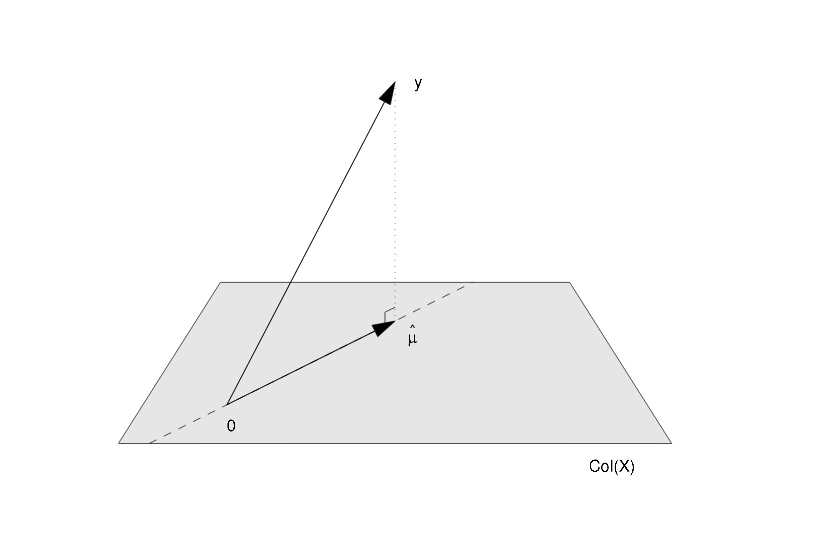
\includegraphics[scale=0.4]{Immagini/spazio-col.png}
%\caption{Rappresentazione dello spazio delle colonne e dei vettori di interesse.}
%\end{figure}
La bontà di adattamento si stima in base a \textit{devianza totale} e
\textit{devianza spiegata}.\\
La \textit{devianza spiegata} è la somma delle differenze al quadrato tra i valori teorici della retta interpolante e la media dei valori empirici.\\
La \textit{devianza residua} è la somma degli scarti al quadrato tra i valori osservati e teorici della $y$. \\
La \textit{devianza totale} è la somma degli scarti dei valori di $y$ empirici dalla loro media.

L'indice di adattamento è definito come:
\begin{equation}
R^2 = \frac{DevSpieg(Y)}{DevTot(Y)}
\end{equation}
Nel caso di un modello di regressione lineare semplice si ha che:
\begin{equation}
DevSpieg(Y) = b_1 Codev(X, Y)
\end{equation}
Dividendo per $n-1$ e con opportuni passaggi (si veda http://www2.stat.unibo.it/montanari/Didattica/lab3.pdf) si arriva a:
\begin{equation}
R^2 = \frac{Cov(X, Y)}{var(X)var(Y)}
\end{equation}

$R^2$ è un numero che varia tra 0 e 1, è = 0 se non c'è correlazione lineare, = 1 se c'è perfetta correlazione.

\subsection{Testare i risultati: t-test e F-measure (test di ipotesi)}
Per testare i risultati ottenuti dei parametri si possono effettuare due misure di test sull'ipotesi nulla che il coefficiente stimato sia o meno uguale a zero, ovvero:
\begin{equation}
H_0 = \beta_i = 0
\end{equation}

\subsubsection{Test di ipotesi e \textit{p-value}}
Un test di ipotesi è un procedimento tramite il quale si verifica la validità di una certa ipotesi. Solitamente si parte definendo un'\textit{ipotesi nulla} tramite la quale si afferma che per la popolazione, o comunque più in generale per il fenomeno che si sta studiando, vale una determinata condizione, ovvero:
\begin{equation}
H_0 = \mu 
\end{equation}
dove $\mu$ sta a indicare una qualsiasi condizione che si vuole testare. \\
L'\textit{ipotesi alternativa} invece specifica che cosa è vero nel caso in cui l'ipotesi nulla sia falsa. La più generale ipotesi alternativa è il contrario dell'ipotesi nulla ovvero:
\begin{equation}
H_1 \neq \mu 
\end{equation}
La valutazione dei risultati di un test di ipotesi avviene considerando il cosiddetto \textit{p-value}. Per calcolare il p-value si calcola prima la distribuzione di probabilità per l'ipotesi nulla, assumendo quindi che essa sia vera si costruisce la distribuzione di probabilità centrata su questo valore, ed in seguito bisogna calcolare la probabilità di ottenere un valore che sia più grande del valore medio osservato per la quantità che si sta studiando. La distribuzione di probabilità che si costruisce infatti è una distribuzione delle  medie, e il valore osservato è una media ottenuta da un campione.\\ 
Il p-value è quindi l'area sottesa alla parte di curva a destra del valore osservato.
Vogliamo che la probabilità evidenziata sia la più piccola possibile, ovvero che il valore osservato sia il più possibile discostato dal centro della curva in quanto essa è centrata sull'ipotesi nulla. Se stabiliamo un livello di confidenza $\alpha$ ciò significa che la \textit{probabilità} di ottenere un valore uguale o più grande del valore osservato deve essere minore o uguale a $\alpha$. Quindi la parte di curva (probabilità) dentro le regioni delle code esterne individuate da $\alpha$ è uguale a $1-\alpha$.
\begin{equation}
P(-Z_{\frac{\alpha}{2}}< \bar{a} < +Z_{\frac{\alpha}{2}}) = 1 - \alpha
\end{equation}
Dove $-Z_{\frac{\alpha}{2}}$ e $+Z_{\frac{\alpha}{2}}$ rappresentano i valori di $\bar{a}$ tali per cui la probabilità racchiusa all'interno di questi valori è uguale a $1-\alpha$. 
\begin{figure}
	\centering
	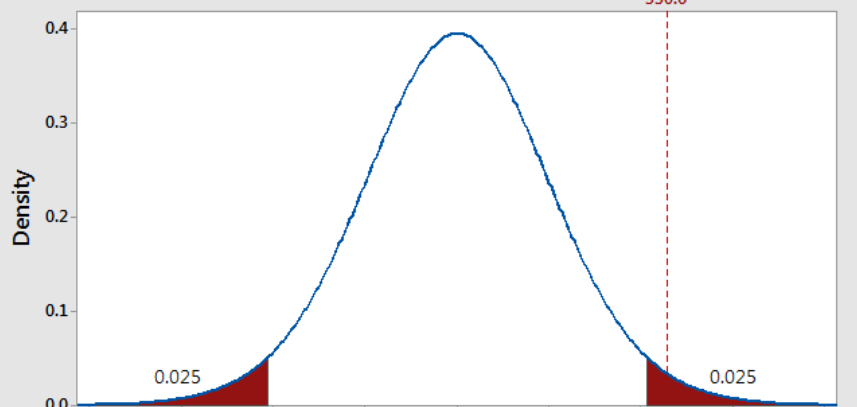
\includegraphics[scale= 0.3]{Immagini/distro-pvalue.png}
	\caption{La curva rappresenta la distribuzione centrata sull'ipotesi nulla, le parti colorate di rosso rappresenta invece il livello $\alpha$ in questo caso uguale al $5\%$, quindi, essendo la curva simmetrica sarà $0,025$ a destra, e $0,025$ a sinistra. La linea tratteggiata rappresenta invece il valore osservato che in questo caso cade all'interno dell'area accettata per rifiutare l'ipotesi nulla.
		credits: http://blog.minitab.com/blog/adventures-in-statistics-2/understanding-hypothesis-tests:-significance-levels-alpha-and-p-values-in-statistics}
	\label{fig: distro-pvalue}
\end{figure}
Se standardizziamo la distribuzione della quantità $\bar{a}$ in modo da renderla a media nulla e varianza 1 (quindi sottraiamo la media e dividiamo per la deviazione standard), otteniamo:
\begin{equation}
P\left(-Z'_{\frac{\alpha}{2}}< \frac{\bar{a} - \mu_a(H_0)}{\sigma} < +Z'_{\frac{\alpha}{2}}\right) = 1 - \alpha
\end{equation}
che implica che $\bar{a}$ deve trovarsi entro i seguenti valori in termini di deviazione standard rispetto alla media:
\begin{equation}
\label{eq: prob-interna}
P\left(\mu_a(H_0) - Z'_{\frac{\alpha}{2}} \cdot \sigma < \bar{a} < \mu_a(H_0) + Z'_{\frac{\alpha}{2}} \cdot \sigma \right) = 1 - \alpha
\end{equation}
I valori di $Z'$ sono tabulati dalla funzione degli errori.\\
La probabilità (p-value) per un valore osservato di $\bar{a}$ è:
\begin{equation}
p = P\left( \left| \frac{\bar{a} - \mu_a(H_0)}{\sigma} \right| > \left| \frac{\bar{a_{oss}} - \mu_a(H_0)}{\sigma} \right| \right)
\end{equation}
che rappresenta quindi la probabilità di osservare un valore di $\bar{a}$ maggiore o uguale a quello che si è osservato (supponendo valida l'ipotesi nulla). Se questo valore di probabilità è inferiore al livello $\alpha$ fissato (quindi il valore $\bar{a_{oss}}$ è al di fuori dell'intervallo individuato in termini di $Z'$ intervalli di confidenza) si può rigettare l'ipotesi nulla.

\begin{tcolorbox}[colback=cyan!5!white, colframe=cyan!75!black, title = Il livello di confidenza $\alpha$]
	A livello interpretativo il livello di confidenza $\alpha$ che si specifica (solitamente è fissato a $0,05$, ovvero al $5\%$ totale della distribuzione) indica la probabilità di rigettare l'ipotesi nulla nel caso in cui poi essa sia effettivamente vera, ovvero le probabilità di errore. Nel valutare l'ipotesi nulla infatti possiamo incappare in due tipi di errori: ritenerla vera quando invece in realtà è falsa, e ritenerla falsa quando invece in realtà è vera. Specificando il livello $\alpha$ stiamo specificando la probabilità di commettere il secondo tipo di errore, infatti se diciamo che rifiutiamo l'ipotesi nulla se il valore che osserviamo cade nelle code, ovvero nella regione $\alpha$ della curva, stiamo comunque rifiutando tutti quei valori della distribuzione per cui l'ipotesi nulla è comunque vera, anche se poco probabile. Quindi nel caso in cui poi l'ipotesi nulla sia effettivamente vera, al massimo in $\alpha \; ( e.g.\!5\%)$ dei casi concluderemo che è falsa, in quanto troveremo i valori nelle code per cui abbiamo deciso si rifiutare l'ipotesi, mentre nel rimanente $95\%$ concluderemo correttamente che è vera. Se invece è effettivamente falsa queste probabilità non valgono più.
\end{tcolorbox}

\subsubsection{t-test}

La \textit{t-statistic}, detta anche \textit{t-measure} o \textit{t-test}, rappresenta un modo per valutare se la stima di una quantità risulta accettabile o meno rispetto ad un'ipotesi nulla. È definita come segue:
\begin{equation}
t = \frac{a - a_0}{SE(a)}
\end{equation}
dove $a_0$ è il valore dell'ipotesi nulla che si sta testando per la quantità $a$ e $SE$  è lo \textit{standard error} di questa variabile ovvero: $\frac{\sigma}{\sqrt{n}}$.\\
Quindi nel caso della stima dei parametri $\beta$ della regressione lineare semplice, in cui per l'ipotesi nulla si suppone che $\beta$ abbia valore zero,  si ha:
\begin{equation}
t = \frac{\beta_i}{SE(\beta_i)} = \frac{\beta_i}{\frac{\sigma}{\sqrt{n \sigma_{jj}}}}
\end{equation}
se la $\sigma$ è nota, altrimenti si usa il suo stimatore $s$, quindi:
\begin{equation}
t = \frac{\beta_i}{\frac{s}{\sqrt{n \sigma_{jj}}}}
\end{equation}
Se si fissa quindi un livello di confidenza $\alpha$ per il p-value,  per esempio $\alpha = 0,05$, si ottiene che l'ipotesi nulla deve essere rigettata se $\vert t \vert > 1,96$. \\
Si può quindi riscrivere il p-value in termini della statistica t:
\begin{equation}
p = P(\vert t \vert > t_{oss})
\end{equation}

Se la quantità $a$ è distribuita normalmente allora t è distribuito come un $\chi^2$ a $n-1$ gradi di libertà che tende ad una distribuzione normale per grandi $n$ (si veda Stock p.87).

\begin{tcolorbox}[colback=cyan!5!white, colframe=cyan!75!black, title= \textbf{Intervallo di confidenza}, sidebyside align=center, lower separated=false]
	Un altro metodo per valutare la validità dell'ipotesi nulla è calcolare l'\textit{intervallo di confidenza} per il valore che si osserva.\\
	Per costruire l'intervallo di confidenza ci si centra sul valore medio osservato e si costruisce su questo una distribuzione campionaria. Secondo l'espressione del t-value, l'ipotesi nulla è rifiutata, secondo un determinato livello di confidenza $\alpha$, se è distante dal valore medio osservato più di t deviazioni standard. Nel caso di $\alpha = 5\%$, si avrà che l'ipotesi nulla non è rifiutata se $-1,96 \cdot SE(\bar{a}) < \bar{a} - \bar{a}_0 < +1,96 \cdot SE(\bar{a})$, ovvero se il valore dell'ipotesi nulla è contenuta all'interno dell'intervallo $[\bar{a} - 1,96 \cdot SE(\bar{a}), \bar{a} + 1,96 \cdot SE(\bar{a})]$ che rappresenta il $95\%$ dei valori della distribuzione campionaria centrata su $\bar{a}$, in quanto è appunto la regione di curva compresa entro 1.96 deviazioni standard.
	\begin{center}
		%\centering
		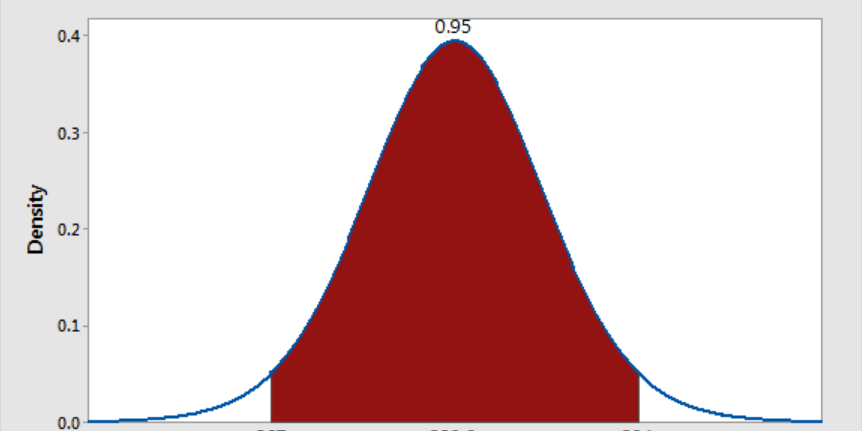
\includegraphics[scale=0.3]{Immagini/intervallo-di-confidenza.png}
		\captionof{figure}{credits: \url{http://blog.minitab.com/blog/adventures-in-statistics-2/understanding-hypothesis-tests\%3A-confidence-intervals-and-confidence-levels}}
	\end{center}
	A questo punto se l'ipotesi nulla è effettivamente vera nel $95\%$ dei casi sarà accettata, mentre solamente nel $5\%$ dei casi sarà rifiutata, cioè per il $95\%$ degli intervalli calcolati per diversi valori osservati sarà accettata, mentre per il rimanente $5\%$ degli intervalli non sarà accettata . Questi intervalli di confidenza sono quelli centrati su valori osservati che sono nella regione del $5\%$ delle code per la distribuzione centrata sull'ipotesi nulla, ovvero quei valori nelle regioni rosse in figura \ref{fig: distro-pvalue}. 
\end{tcolorbox}

\subsubsection{F measure}
Nel caso sia condotta una regressione con più regressori si può effettuare un test di ipotesi congiunto per i vari parametri che vengono stimati, ovvero vedere se un determinato set di parametri è efficiente o meno nella stima del modello. Quindi è definita la seguente ipotesi nulla:
\begin{equation}
\begin{split}
H_0 &: \; \beta_0 = \beta_1 = \dots = \beta_k = 0 \\
\end{split}
\end{equation}
che implica l'ipotesi alternativa:
\begin{equation}
H_1: \; \beta_0 \neq 0 ,\; \beta_1 \neq 0,\; \dots ,\; \beta_k \neq 0
\end{equation}
ovvero si testa se uno tra i parametri stimati sia nullo, se si rifiuta l'ipotesi nulla significa che almeno uno di essi non è nullo, e quindi è significativo.

Il test di ipotesi congiunta si effettua calcolando la F-measure per il modello lineare preso in esame, definita come segue:
\begin{equation}
F = \frac{SSR_r - SSR_{ur}/q}{SSR_{ur}/(n-(k+1))}
\label{F-measure}
\end{equation}
Dove:
\begin{itemize}
	\item $SSR$ rappresenta la somma dei residui al quadrato del modello, cioè la devianza residua.
	\subitem In particolare $SSR_r$ rappresenta la devianza residua per il modello ristretto all'ipotesi nulla, in cui i parametri sono posti pari ai valori specificati dall'ipotesi (in questo caso zero).
	\subitem $SSR_{ur}$ rappresenta invece la devianza residua per il modello non ristretto, ovvero quello stimato con tutti i parametri.
	\item La variabile $q$ rappresenta invece il numero di restrizioni, ovvero il numero di parametri che sono testati congiuntamente.
	\item $n$ rappresenta il numero di osservazioni nel campione.
	\item $k$ il numero di variabili indipendenti nel modello non ristretto.
\end{itemize}
Le due quantità rapportate nell'equazione \eqref{F-measure} sono distribuite come un $\chi^2$ che implica che la $F$ sia distribuita come una F di Fisher-Snedecor con $q$ e $n-(k+1)$ gradi di libertà. Possiamo quindi impostare un livello di significatività $\alpha$ con il quale rifiutare l'ipotesi nulla. L'ipotesi nulla è accettata se:
\begin{equation}
P(F_0 < F_\alpha) = 1-\alpha
\end{equation}
ovvero se si ottiene un valore per il test $F_0$ minore del valore $F_\alpha$, valore per cui la probabilità è uguale a $1-\alpha$. Questo valore si può trovare tabulato. Se invece si trova un valore maggiore, tale per cui la probabilità di ottenere un valore maggiore o uguale è uguale o minore di $\alpha$, allora si può rigettare l'ipotesi nulla.
\subsection{Stima dei parametri tramite massima verosimiglianza}
Nel modello lineare classico gli errori si distribuiscono, come si è detto, in modo gaussiano, ovvero:
\begin{equation}
\epsilon_i \sim N(0,\sigma^2)
\end{equation}
così come anche i parametri e le variabili dipendenti, cioè:
\begin{equation}
\begin{split}
b_{OLS} &\sim N(\beta, \sigma^2(X^tX)^{-1}) \\
Y &\sim N(X\beta, \sigma^2 I_n)
\end{split}
\end{equation}
Si può quindi provare a utilizzare stime di massima verosimiglianza che chiedono l'esistenza di n variabili casuali $y_i - X_i\beta$ con $i=1 \cdots n$ che siano identicamente e indipendentemente distribuite condizionatamente al valore $X$ e dipendenti dai parametri $\beta$.\\
Si cerca quindi il valore dei parametri che rendono massima la probabilità di ottenere la verosimiglianza massima:
\begin{equation}
max_\beta L(y_i - X_i\beta) \quad i=1 \cdots n
\end{equation}
Da questo si arriva a dimostrare che lo stimatore dei $\beta$ di massima verosimiglianza (ML) coincide con quello trovato in precedenza, e possiede le stesse proprietà di consistenza, correttezza ed efficienza, comprese le proprietà asintotiche richieste nel caso in cui le misure siano statisticamente indipendenti.

\subsection{Variabili esplicative qualitative}
Le variabili esplicative qualitative o categoriche sono determinate da attributi:
\begin{itemize}
	\item nominali
	\item ordinali
\end{itemize}
e possono essere:
\begin{enumerate}
	\item dicotomiche (\textit{dummy variables}) se assumono solamente due valori (e.g. sesso);
	\item Politomiche, se assumono più di due valori.
\end{enumerate}

Ora se abbiamo un modello lineare del tipo:
\begin{equation}
Y_i = \beta_0 + \beta_1 D_i + \epsilon_i \quad i=1 \cdots n
\end{equation}
in cui la $D_i$ è una variabili dummy, si ha che essa va ad esercitare il proprio effetto sull'intercetta. Solitamente si riconducono le due possibilità per la variabile dummy ai due valori 0 e 1, per cui quando si ha $D=0$ si ottiene:
\begin{equation}
Y_i = \beta_0 + \epsilon_i
\label{eq: dummy intercetta}
\end{equation}
mentre quando $D=1$, si ottiene:
\begin{equation}
Y_i = \beta_0 + \beta_1 + \epsilon
\label{eq: dummy completa}
\end{equation}
ovvero l'intercetta rappresenta il \textit{valore stimato} di $Y$ quando la variabile esplicativa dummy è uguale a 0. Il coefficiente angolare è dato invece dalla differenza in Y per i due diversi valori della variabile esplicativa dummy, ovvero facendo la differenza tra la \eqref{eq: dummy intercetta} e \eqref{eq: dummy completa}.
La statistica inferenziale si fa anche in questo caso come prima, utilizzando stime e test.

\chapter{Violazioni del Modello Lineare Classico}

\subsection{Eteroschedasticità}
L'ipotesi di omoschedasticità suppone che il termine di errore sia uguale per tutte le variabili indipendenti, quindi dato un certo valore di X lo spread nella distribuzione delle Y è sempre lo stesso, come si può vedere dalla figura \ref{fig:regressione-omoschedastica}.
\begin{figure}[H]
	\centering
	\makebox[\textwidth]{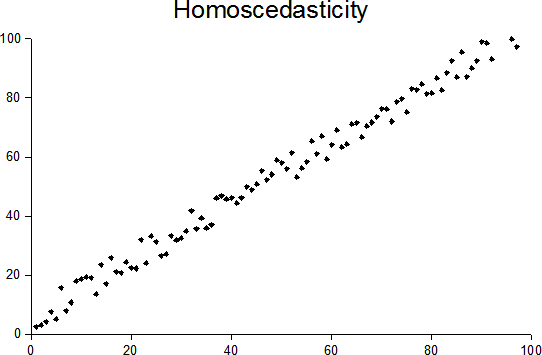
\includegraphics[width=0.8\textwidth]{Immagini/Homoscedasticity.png}}
	\caption{Regressione lineare con distribuzione omoschedastica degli errori.}
	\label{fig:regressione-omoschedastica}
\end{figure} 
ovvero $Var(\varepsilon \vert x_i) = \sigma^2$ e $E(y \vert x) = 0$.

Al contrario ci possono essere situazioni in cui il termine di errore varia tra le diverse variabili indipendenti, ottenendo così la situazione mostrata in figura \ref{fig:regressione-eteroschedastica}
\begin{figure}[H]
	\centering
	\makebox[\textwidth]{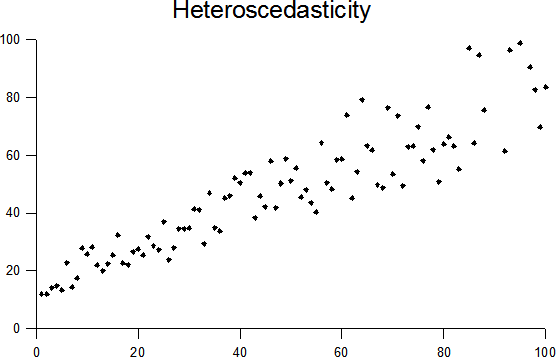
\includegraphics[width=\textwidth]{Immagini/Heteroscedasticity.png}}
	\caption{Regressione lineare con distribuzione eteroschedastica degli errori.}
	\label{fig:regressione-eteroschedastica}
\end{figure} 
Questo andamento è conseguenza del fatto che la varianza del termine di errore, stimato dai residui del modello, dato un certo valore di X non è più costante e in particolare ora dipende da X.

Un altro andamento anomalo del tipo in figura \ref{fig: residui-eteroschedastici} lo si può osservare in un semplice grafico scatter plot della variabile dipendente in funzione della variabile indipendente: nel caso di errori omoschedastici i punti sono collocati in modo equidistante dalla retta interpolante, mentre nel caso di errori eteroschedastici i punti sono distanziati in maniera diversa da questa. Il problema nel caso eteroschedastico si pone in quanto il metodo OLS dei minimi quadrati ordinari mira a minimizzare i residui ottenendo lo standard error minimo. Il metodo OLS pesa però tutte le osservazioni allo stesso modo, mentre quando si trattano errori eteroschedastici è necessario pesare meno i valori con più errore e pesare di più quelli che invece sono più rilevanti.\\
Se utilizziamo ancora stimatori OLS cosa succede?\\
$\rightarrow$ Gli stimatori OLS dei parametri sono ancora unbiased, consistenti e distribuiti in modo asintoticamente normale. \textit{Non} sono più stimatori \textit{efficienti} tra tutti gli stimatori possibili dei parametri che sono lineari e unbiased in $Y$, dato un certo valore di $X$. In generale quindi possiamo dire che non sono più BLUE (Best Linear Unbiased Estimator).
La statistica t di Student calcolata in base al valore della deviazione standard utilizzato nel metodo OLS, non risulta più distribuita in modo normale nemmeno per grandi campioni se l'errore è eteroschedastico. Questo avviene principalmente per due ragioni:
\begin{enumerate}
	\item Le stime campionare tendono a sottostimare il valore della varianza.
	\item Non c'è più da calcolare una sola varianza ma diverse varianze.
\end{enumerate}
Come conseguenza della sottostima della varianza si ha che la statistica t di Student ha valori erroneamente elevati, si possono considerare come significativi paramentri che in realtà non lo sono. Per lo stesso motivo la regione di accettazione diventa molto più piccola di quanto non lo sia in realtà e di conseguenza la regione di rifiuto molto grande.
L'ipotesi di omoschedasticità (uguali varianze) è  infatti alla base di test come l'analisi della varianza ANOVA (Analysis Of Variance) e il t-test di Student.
\begin{tcolorbox}[colback=cyan!5!white, colframe=cyan!75!black, title = ANOVA]
	L'analisi della varianza ANOVA è utilizzata per testare differenze tra medie, utilizzando appunto le varianze. Quando le medie sono solamente due è indifferente utilizzare questo test oppure il t-test, mentre si deve usare necessariamente il test ANOVA quado le medie da testare sono più di due.\\
	Dati quindi un insieme di campioni di cui sono stati calcolati media e varianza per ciascuno si può procedere a costruire il test ANOVA, come segue:
	\begin{equation}
	F = \frac{\sigma^2_{between}}{\sigma^2_{within}}
	\label{eq: test ANOVA}
	\end{equation}
	dove $\sigma^2_{between}$ rappresenta la varianza tra gruppi, mentre $\sigma^2_{within}$ quella in gruppi.\\
	La varianza $within$ in gruppi è la media delle varianze di ciascun campione pesata sul numero di gradi di libertà del campione, overo:
	\begin{equation}
	\sigma^2_{within} = \frac{1}{a(n-1)}\sum_{i=1}^{a}\sum_{j=1}^{n}(y_{ij} - \bar{y_i})^2
	\end{equation}
	in cui appunto la $i = 1 \cdots a$ identifica il campione e $j = 1 \cdots n$ identifica invece il numero di osservazione che si sta prendendo in considerazione. Quindi si somma prima su $j$ per calcolare le varianze del campione che si sta considerando, e poi si somma su $j$ per fare la media delle varianze dei campioni, dividendo poi per il peso del campione pari a $n-1$, dove $n$ è il numero delle osservazioni fatte per campione. \\
	La varianza $between$ tra gruppi invece è calcolata a partire dalla devianza totale che è la varianza stimata con tutte le osservazioni di tutti i campioni ovvero come se le varie osservazioni dei vari campioni appartenessero tutte ad un unico campione. A questo punto la varianza tra gruppi si ottiene moltiplicando questa per $n$, ovvero:
	\begin{equation}
	\sigma^2_{between} = \frac{n}{a-1}\sum_{i=1}^{a} (\bar{y_i} - \bar{\bar{y}})
	\end{equation}
	dove $\bar{\bar{y}}$ rappresenta appunto la media ottenuta considerando le osservazioni di tutti i campioni, mentre le $\bar{y}_i$ sono le medie dei singoli campioni.	
	Si può quindi a questo punto effettuare il test in \eqref{eq: test ANOVA}. Poichè le due varianze rapportate sono stime di una stessa varianza parametrica (quella della distribuzione vera se si conoscesse tutta la popolazione), allora questo rapporto deve essere uguale a 1 in teoria. Se però i campioni provengono da popolazioni diverse si ottiene un valore al numeratore più grande rispetto al denominatore, risultando così in un numero maggiore di 1.\\
	Per ogni combinazione di gradi di libertà di numeratore e denominatore, si confronta il valore ottenuto con la distribuzione di una variabile casuale distribuita come una F di Sendecor con pari gradi di libertà. Stabilendo il livello di confidenza, si confronta con il valore tabulato della $F$ e si decide se confermare l'ipotesi nulla, cioè che le medie provengono tutte da una stessa distribuzione, oppure se rigettarla, affermando quindi che almeno una non appartiene alla distribuzione delle altre.	
	[ref:http://docenti.unimc.it/monica.raiteri/teaching/2013/12316/files/slides-i-parte-per-studenti-frequentanti/interpretazione-del-test-f-distribuzione-f-di]
\end{tcolorbox}
Oltre alla visualizzazione grafiche, l'eteroschedasticità si può individuare anche tramite metodi analitici, ovvero eseguendo dei test come il \textit{test di White} o il \textit{test di Breusch-Pagan}.
\subsubsection{Test di White}
Il test di White testa l'ipotesi nulla di omoschedasticità degli errori:
\begin{equation}
H_0 = Var(\epsilon \vert X) = \sigma^2 \cdot I_n
\end{equation}
e ovviamente ha come ipotesi alternativa la stessa espressione sopra in cui vale però una disuguaglianza.
Il test di White si basa su na regressione OLS dei residui, ovvero:
\begin{enumerate}
	\item si stima il modello lineare con il metodo OLS ottenendo:
	\begin{equation}
	\hat{Y_i} = \hat{\beta_0} + \hat{\beta_1} \cdot X_{i1} + \cdots + \beta_n \cdot X_{in} + \hat{\epsilon_i}
	\end{equation}
	\item si fa una regressione OLS  sugli errori assumendo che l'eteroschedasticità possa essere una funzione lineare dei regressori, del loro quadrato o della loro interazione $x_{ij}\cdot x_{ij}$. Quindi si ottiene:
	\begin{equation}
	\hat{\epsilon}_i^2 = \delta_0 + \delta_1 \hat{Y}_i + \delta_2 \hat{Y}_i^2
	\end{equation}
	dove appunto si utilizza il risultato della regressione del modello lineare effettuato all'inizio. Considerando i quadrati si considerano tramite i doppi prodotti anche i termini di interazione.
	\item si calcola $R^2_{\hat{\epsilon}_i^2}$
	\item si effettua il test LM, definito come segue:
	\begin{equation}
	LM = nR^2_{\hat{\epsilon}_i^2}
	\end{equation}
	che si distribuisce come un $\chi^2$ con un numero di gradi di libertà pari al numero di regressori inseriti nel modello.
	\item scelto un livello di significatività $\alpha$ l'ipotesi nulla sarà rigettata se il test $LM$ risulta superiore al valore soglia di $\chi^2$ (tabulato), che è associato al livello di significatività scelto.
\end{enumerate}
\subsubsection{Test di Breusch-Pagan}
Il test di Breuch Pagan a differenza del test di White ipotizza che l'eteroschedasticità sia solamente una funzione lineare delle variabili indipendenti, trascurando quindi i termini quadratici e di interazione. Si procede quindi nello stesso modo definito precedentemente in cui però si assume che la forma funzionale per $\epsilon$ sia:
\begin{equation}
\hat{\epsilon}_i^2 = \delta_0 + \delta_1\hat{Y}_i
\end{equation}
CHIEDERE..
\subsection{Autocorrelazione}
A volte è possibile che gli errori (e quindi i residui) siano correlati tra loro, soprattutto in serie storiche o territoriali è ragionevole ipotizzare che ci sia correlazione tra gli errori che vengono stimati in momenti successivi o territori vicini.\\
Nel modello lineare classico si suppone che:
\begin{equation}
Cov(\varepsilon_i, \varepsilon_j) = 0 \quad \forall i \neq j
\end{equation}
Quando ciò non si verifica si dice che gli erroi sono correlati o che si è in presenza di una correlazione seriale. Se c'è omoschedasticità ma c'è correlazione, la matrice degli errori è:
\begin{equation}
\Sigma = \begin{pmatrix}
\sigma^2 & \rho_{1,2} & \cdots & \rho_{1,n} \\ 
\rho_{1,2} & \sigma^2 & \cdots & \vdots \\ 
\vdots &  & \ddots & \vdots \\ 
\rho_{1,n} & \cdots & \cdots & \sigma^2
\end{pmatrix} 
\end{equation}
dove i vari $\rho$ rappresentano i termini di correlazione dei vari termini di errore tra loro. La matrice ovviamente risulta simmetrica.
L'errore può essere correlato con quello dell'osservazione immediatamente precedente e quindi avere una correlazione di primo livello, oppure ci può essere una correlazione di secondo livello o livello maggiore se gli errori correlati sono distanti due o più osservazioni. Ciò è espresso con la seguente formula:
\begin{equation}
\varepsilon'_i = \varepsilon'_{i-1} + \eta_j
\end{equation}
dove si è utilizzata la notazione primata per identificare il fatto che gli errori sono correlati tra loro e non sono più sferici. Gli $\eta_j$ sono invece identicamente e indipendentemente distribuiti in modo normale con $N(0,\sigma_i)$ per rappresentare quindi la parte di correlazione dell'errore con sè stesso (la diagonale della matrice).\\
Si ha autocorrelazione \textit{positiva} quando residui consecutivi tendono ad essere dello stesso segno e simili in valore, \textit{negativa} quando invece residui consecutivi sono di segno differente.
IMMAGINI AUTOCORRELAIZONE POSITIVA E NEGATIVA
In caso di autocorrelazione gli stimatori OLS  dei parametri per la regressione lineare sono ancora lineari e corretti (unbiased) ma non sono più i migliori stimatori possibili, quindi non sono più BLUE, ovvero esistono altri stimatori che risultano più efficienti. come conseguenza di ciò non si potrà più usare la varianza campionaria nella statistica $t$ perchè non potrà più approssimare la varianza vera in quanto la $t$ è costruita supponendo l'incorrelazione degli errori nella popolazione e il valore atteso della varianza campionaria non stima correttamente la varianza vera. Di conseguenza la statistica $t$ assume valori erroneamente elevati, considerando significativi parametri quando in realtà non lo sono, ovvero si amplia la regione di rifiuto per l'ipotesi nulla con il conseguente restringimento della regione di accettazione. \\
Ragionamenti analoghi si possono fare per il test F, che corrisponde semplicemente al quadrato del t test.
\subsubsection{Individuazione grafica}
Si può notare un autocorrelazione nei reisui osservando:
\begin{enumerate}
	\item scatter plot della vraibile dipendente in funzione in funzione del regressore $x$. Nel caso in cui ci fossero più regressori bisogna fare uno scatter plot in funzione di goni regressore. Se si nota una certa regolarità nell'andamento allora si è in presenza di correlazione.
	\item scatter plot dei residui in funzione del regressore: anche qui valgono le stesse considerazioni fatte sopra. Se i residui oscillano intorno allo zero non c'è correlazione.
	\item Residui in funzione dei residui ritardati
	\item Correlogramma, permette di identificare chiaramente quali sono i gradi di correlazione che influiscono di più. Solitamente nei correlogramma è mostrata anche una banda di confidenza che indica il limite entro il quale non si ritiene che vi sia autocorrelazione. Se il coefficiente di autocorrelazione che si sta valutando esce da questa banda allora si è in presenza di autocorrelazione.
\end{enumerate}
\subsubsection{Test di Durbin-Watson}
Il test di Durbin-Watson verifica l'ipotesi nulla:
\begin{equation}
H_0:\; \rho = Corr(\varepsilon'_i, \varepsilon'_{i-1}) = 0
\end{equation}
dove $\varepsilon'_i$ e $\varepsilon'_{i-1}$ sono i residui relativi all'osservazione i-esima e i-1-esima.\\
La statistica di DW con cui si effettua il test è la seguente:
\begin{equation}
DW = \frac{\sum_{i}(\varepsilon'_i - \varepsilon'_{i-1})^2}{\sum_{i} \varepsilon'^2_{i}} \quad \text{per}\; i = 1 \dots n
\label{eq: DW test}
\end{equation}
La statistica di DW è centrata su 2 ed è sempre compresa tra 0 e 4. Nel caso in cui i residui siano correlati positivamente tende a 0, mentre nel caso in cui siano correlati negativamente tende a 4.\\
Non si conosce la distribuzione teorica di questa statistica, comunque esistono dei valori tabulati in base al numero di regressori, il numero di osservazioni e livello di significatività con cui si vuole valutare l'ipotesi nulla, con in quali è possibile individuare dei valori critici $d_l$ e $d_u$ che delimitino le regioni di rifiuto e di accettazione. Se il valore che si trova dalla statistica in \eqref{eq: DW test} è $d < d_l$ allora si può concludere che c'è autocorrelazione positiva, se $d > d_u$ allora si può concludere che c'è autocorrelazione negativa, mentre se $d$ è compreso tra questi due valori allora non c'è sufficiente evidenza per concludere che ci sia autocorrelazione tra i residui. Convenzionalmente, nel caso in cui i valori di $d_l$ e $d_u$ non vengano specificati si fissa $d_l = 1$ e $d_u = 3$.
\section{WLS e GLS}
Per tenere conto di eteroschedasticità e correlazione nei residui si possono applicare due metodi: il metodo dei minimi quadrati pesati WLS e il metodo dei minimi quadrati generalizzati GLS.
\subsection{Il metodo WLS}
Per tenere conto dell'eteroschedasticità, e fare in modo che i valori stimati dei parametri $\hat{\beta}$ siano ancora gli stimatori migliori, è stato dimostrato che tali stimatori risultano ancora i migliori se si minimizza una somma pesata dei residui dove i pesi sono il reciproco dello scarto quadratico medio per i valori previsti, ovvero:
\begin{equation}
S = \sum_{i=1}^{n} \sqrt{W_{ii}} r_i^2 \quad \text{dove}\quad W_{ii} = \frac{1}{\sigma_i^2} 
\label{eq: somma-gls}
\end{equation}
per poi procedere con la minimizzazione come nel caso OLS. \\
Alternativamente al posto di definire la \eqref{eq: somma-gls} si può effettuare un cambiamento di variabili per il modello lineare classico, ovvero passare da:
\begin{equation}
Y = X\beta + \varepsilon^\star
\label{eq: regressione-lineare-eterosched}
\end{equation} 
dove $\varepsilon^\star$ indica l'errore eteroschedastico, a:
\begin{equation}
Y^\star = X^\star\beta + \varepsilon
\end{equation}
dove:
\begin{equation}
\begin{split}
Y^\star &= \frac{Y}{\sqrt{W_{ii}}} \\
X^\star &= \frac{X}{\sqrt{W_{ii}}} \\
\end{split}
\end{equation}
ovvero si dividono entrambi i membri dell'equazione OLS per $W_{ii}$ e poi si procede con il metodo dei minimi quadrati ordinari. Questa volta l'errore risulta omoschedastico, in quanto abbiamo diviso per la devianza standard della media anche la parte di errore, quindi la diagonale della matrice di correlazione REFF A UNA MATRICE PRECEDENTE DI CORRELAZIONE DEI RESIDUI NEL CASO DI ERRORI ETEROSCHED (FARLA NEL CASO MANCHI) dei residui non è più composta da termini tutti diversi tra loro ma saranno tutti uguali e costanti.
\subsection{Il metodo GLS}
Anche il metodo GLS, di cui il metodo WLS è un caso particolare, si basa su una trasformazione di variabili.
Data la matrice di varianza e covarianza per gli errori del modello lineare classico, caratterizzata, nel caso di errori omoschedastici ma correlati, da una diagonale tutta uguale e con termini diversi da zero fuori dalla diagonale, si supponga che esista una matrice $V$ tale che:
\begin{equation}
\Sigma_{\varepsilon^\circ} = V \sigma^2 V^t
\label{eq: matrice-GLS}
\end{equation}
o analogamente:
\begin{equation}
\Sigma_{\varepsilon^\circ}^{-1} = (V)^{-1} \frac{1}{\sigma^2} (V^t)^{-1}
\end{equation}
dove si è usata la notazione $\varepsilon^\circ$ per indicare che gli errori sono correlati.\\
Si possono definire gli errori trasformati, fatti nel seguente modo:
\begin{equation}
\varepsilon = V^{-1} \varepsilon^\circ
\end{equation}
poichè vale la \eqref{eq: matrice-GLS}, allora si ottiene:
\begin{equation}
\Sigma_\varepsilon = VV^{-1} \sigma^2 (V^t)^{-1}V^t = \sigma^2 \cdot I_n
\end{equation}
A questo punto se passiamo sin da subito a delle variabili trasformate nel modello, moltiplicando a entrambi i membri l'equazione del modello lineare classico in \eqref{eq: regressione-lineare-eterosched}, considerando di avere questa volta errori autocorrelati omoschedastici, per $V^{-1}$, si può applicare il metodo OLS classico per ottenere i parametri.
La matrice $V$ si può ottenere tramite decomposizione spettrale della matrice $\Sigma_\varepsilon$ di correlazione degli errori.
Lo stimatore GLS che si calcola in questo modo assegna un peso maggiore alle variabili caratterizzate da una minore varianza e quindi da considerarsi più attendibili. Inoltre lo stimatore è consistente, corretto (unbiased) e per il terorema di Aitken (analogo al Gauss-Markov per gli OLS) si dimostra che è anche efficiente.
\subsubsection{Procedimento}
Prima di procedere alla costruzione delle stime GLS,  si deve stimare il l'errore autocorrelato e i vari livelli di autocorrelazione. A questo scopo si costruisce un modello di regressione che spiega l'errore $\varepsilon_i$ per l'osservazione i-esima in termini delle variabili esplicative e del residuo ritardato $\varepsilon_{i-1}$, ovvero:
\begin{equation}
\varepsilon^\circ = a_0 + a_1x_1 + \cdots + a_n x_n + a_\varepsilon \varepsilon_{i-1}^\circ
\end{equation}
Il coefficiente di regressione $a_\varepsilon$ che si ottiene rappresenta una stima per il coefficiente $\rho$ di autocorrelazione al primo ordine.
COSA DEL SOTTRARRE (slide 78-79 violazione errori.pptx)
Alternativamente a questo metodo si può utilizzare un metodo autoregressivo che introduce tre le variabili esplicative anche un termine di errore ritardato che tenga conto dell'autocorrelazione al primo ordine. Se ci sono correlazioni anche a ordini successivi si introducono tante variabili esplicative che ne tengano conto in un numero pari agli ordini che si considerano.
\subsection{Il metodo FLGS}
Il problema del metodo GLS è che si basa su una conoscenza perfetta della matrice $\Sigma_\varepsilon$ che però non sempre è nota, per questo si usa il metodo FGLS che si basa sulla matrice di varianza e covarianza campionaria. Gli stimatori che si calcolano con il FGLS sono consistenti nel senso che per $N \rightarrow +\infty \; \Rightarrow \; S_\varepsilon \rightarrow \Sigma_\varepsilon$, dove $S_\varepsilon$ indica la matrice di varianza e covarianza per gli errori campionaria.
\textit{Oss.}\\
Poichè il WLS è un caso particolare del GLS, tutte le procedure che si usano nel GLS si possono adottare anche nel WLS. 

\section{Multicollinearità}
Abbiamo costruito lo stimatore dei minimi quadrati tramite l'equazione \ref{eq:2.21}, in cui la matrice $ \left(\doubleunderline{X}^T \doubleunderline{X}\right) $ dev'essere invertibile. Nel caso non lo fosse, o avesse determinante prossimo allo zero, le stime della regressione non potrebbero essere ottenuta, o perchè non esistono sufficienti dati per ottenerle, oppure perchè sono empiricamente sottostimate dal modello. In questi casi si dice che nel modello esiste multicollinearità tra le variabili esplicative, che può avere due forme:
\begin{itemize}
	\item Multicollinearità imperfetta: quando due o più variabili esplicative usate per costruire il modello sono fortemente correlate tra loro. In questo caso la matrice di cui sopra ha determinante tanto più prossimo allo zero quanto più alta la correlazione tra le variabili.
	\item Multicollinearità perfetta: quando una variabile esplicativa è combinazione lineare di altre variabili. In questo caso la matrice ha determinante nullo.
\end{itemize}

\section{Regressione logistica}
[ref: https://codesachin.wordpress.com/2015/08/16/logistic-regression-for-dummies/ , https://www.youtube.com/watch?v=gNhogKJ\_q7U]\\
La regressione logistica a differenza di altri tipi di regressione non si pone l'obiettivo di predire il valore di una variabile dato un certo numero di input. La regressione logistica si applica infatti a variabili categoriche. La regressione logistica restituisce in output la \textit{probabilità} che un certo punto in input appartenga ad una certa classe. Assumiamo per semplicità di avere solamente due classi (classe binaria) in cui la variabile dipendente $y$ può assumere valori. A differenza della regressione lineare classica quindi la variabile dipendente può assumere solamente un numero finito di valori e non uno spettro continuo. Possiamo comunque provare ad applicare una regressione lineare ad un problema che coinvolge variabili questo tipo, infatti a parte essere una variabile binaria, non c'è nulla di speciale nella variabile y che vogliamo prevedere, i problemi sorgono quando si devono poi interpretare i risultati restituiti da questo modello. Applichiamo quindi un modello lineare utilizzando tutte le variabili indipendenti $x_1, \cdots, x_n$ che si ritengono significative per la previsione di un'uscita della variabile $y$. Sia questa uscita $y=1$, più il risultato restituito dal modello, per determinati valori delle variabili indipendenti, è alto, più sarà probabile che il valore per la variabile dipendente sia effettivamente uguale a $1$. Per esempio possiamo considerare il caso di superare o meno un esame, la possibilità di successo la codifichiamo con il valore $y=1$, mentre quella di insuccesso con il valore $y=0$. Per convenzione solitamente si predice la variabile che viene indicata con $1$, quindi in questo caso la possibilità di successo, di conseguenza inseriamo nel modello tutte quelle variabili che riteniamo significative per questa predizione. Supponendo di avere tra le variabili solamente il tempo di studio il modello lineare avrà la seguente forma:
\begin{equation}
y = \beta_0 + \beta_1\cdot tempo\;di\;studio
\label{eq: esempio-regressione-lineare-logistica}
\end{equation}
dai risultati di questa predizione otterremo dei valori per i coefficienti che vengono stimati tramite maximum likelihood (per approfondire si veda https://onlinecourses.science.psu.edu/stat504/node/150) ma cosa significa il risultato di questa regressione. Supponiamo per esempio di ottenere come risultati $\beta_0 = -1$ e $\beta_1 = 2$, se consideriamo un tempo di studio pari a 2 ore e lo inseriamo all'interno dell'equazione otteniamo per la variabile $y$, che in questo caso rappresenta la possibilità di superare l'esame, un valore pari a 1, ma cosa indica? Così com'è per ora non indica nulla, infatti se volessimo interpretarlo come la probabilità di superare l'esame sbaglieremmo in quanto quest'ultima deve sempre risiedere tra 0 e 1, mentre in questo caso se per esempio consideriamo un tempo di studio di 5 ore per esempio otteniamo un valore negativo, e se scegliamo il caso in cui il tempo di studio sia nullo si ottiene per $y$ un risultato negativo. Per poter passare dai risultati della regressione lineare a delle probabilità $P$ è necessario applicare una trasformazione non lineare che:
\begin{enumerate}
\item Assuma sempre valori positivi
\item Sia compresa tra 0 e 1
\end{enumerate} 
Per soddisfare il primo punto si applica una funzione esponenziale all'espressione della regressione lineare quindi dalla \eqref{eq: esempio-regressione-lineare-logistica}, che più in generale può essere riscritta come $y = \beta_0 + \beta_1 \cdot x_1 + \beta_2 \cdot x_2 + \cdots$, si passa a:
\begin{equation}
P = \exp(\beta_0 + \beta_1 \cdot x_1 + \beta_2 \cdot x_2 + \cdots)
\end{equation}
Ora è necessario che $P$ sia compresa risulti minore di $1$, in quanto con il passaggio precedente ci assicuriamo già che assuma solo valori positivi. Per fare ciò ci basta divider l'espressione precedentemente ricavata per un numero che sia leggermente più grande, di modo da ottenere così una funzione che tenda asintoticamente a $1$ e a $0$. Per fare questo dividiamo per la stessa quantità a cui sommiamo $1$, ottenendo così l'espressione per la probabilità:
\begin{equation}
P = \frac{\exp(y = \beta_0 + \beta_1 \cdot x_1 + \beta_2 \cdot x_2 + \cdots)}{\exp(y = \beta_0 + \beta_1 \cdot x_1 + \beta_2 \cdot x_2 + \cdots) + 1}
\end{equation}
L'interpretazione del modello lineare si può però ancora mantenere in quanto:
\begin{equation}
\log(\frac{P}{1-P}) = \beta_0 + \beta_1 \cdot x_1 + \beta_2 \cdot x_2 + \cdots
\label{eq: logit}
\end{equation}
dove $1-P$ oltre a permettere il passaggio per ottenere l'espressione lineare, dal punto di vista interpretativo rappresenta la probabilità di ottenere $y = 0$. A volta ci si riferisce al rapporto $\frac{P}{1-P}=\frac{P(y=1)}{P(y=0)}$ con il termine di \textit{Odds ratio}. Quando viene applicata la regressione logistica viene applicata la formula \eqref{eq: logit}, detta anche \textit{logit}, per cui per ottenere i valori di probabilità associati a determinati valori delle variabili indipendenti che si sono utilizzate è necessario applicare la formula inversa.
nei software è spesso anche possibile impostare una soglia per la probabilità con la qual stabilire e quindi predire se una certa osservazione con una certa probabilità appartenga ad una determinata classe. In questo modo si possono poi calcolare delle contingency table dalle quali vedere quanti valori sono stati correttamente predetti e quanti invece no.


\end{document}
